\documentclass[11pt, oneside]{article} 
\usepackage{geometry}
\geometry{letterpaper} 
\usepackage{graphicx}
	
\usepackage{amssymb}
\usepackage{amsmath}
\usepackage{parskip}
\usepackage{color}
\usepackage{hyperref}

\graphicspath{{/Users/telliott/Github/calculus_book/png/}}
% \begin{center} 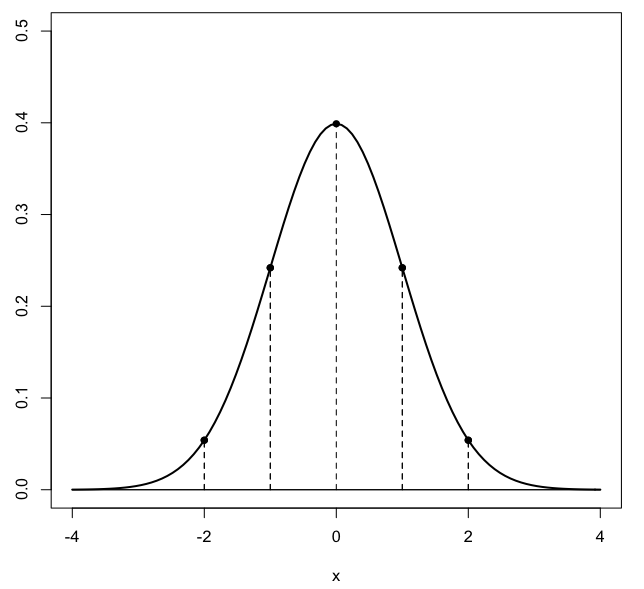
\includegraphics [scale=0.4] {gauss3.png} \end{center}

\title{Induction}
\date{}

\begin{document}
\maketitle
\Large

\label{sec:Induction}

\subsection*{the problem}

Suppose we have some theorem that we think \emph{might be true} for all numbers $n$, because we've tried it on a few different values of $n$ and the theorem is true for all of them.  

A classic example (Courant and Robbins) is this prime number generator:
\[ p(n) = n^2 - n + 41 \]

The remarkable function $p(n)$ produces a prime number for integer $0 < n < 41$.

\begin{verbatim}
  41   43   47   53   61   71   83   97
 113  131  151  173  197  223  251  281
 313  347  383  421  461  503  547  593
 641  691  743  797  853  911  971 1033
1097 1163 1231 1301 1373 1447 1523 1601
1681
\end{verbatim}

But, for $n=41$, the last two terms cancel in
\[ p(n) = n^2 - n + 41 \]

 and then $n^2$ is divisible by $n$, thus the result cannot be prime.

By testing them all, I found that $41$ is the largest prime smaller than $2000$ with this property (I don't know of a proof that no more exist).  The known primes with this property are:

\begin{verbatim}
 2  3  5 11 17 41
\end{verbatim}

Hamming has some other examples of theorems with many true candidates, but which are false.  Here is one:
\[ f(n) = n(n-1)(n-2) \dots (n-k) \]
$f(n)=0$ for all $0 \le n \le k$, but will never be zero for any other $n > k$.  That is because there are only $k$ zeroes of a kth degree polynomial.  (As an aside, this is a consequence of the \emph{fundamental theorem of algebra}).

By choosing $k$ large, we can generate as many true cases as you like.

Furthermore, for any function $g(n)$, $f(n) + g(n)$ will have the same property.

\subsection*{induction}

\subsection*{induction in geometry}

In the figure below is a polygon---an irregular heptagon.  Actually, there are three polygons altogether, there is the heptagon with $n+1$ sides, the hexagon with only $n$ sides that would result from cutting along the dotted line, and the triangle that is cut off.

We want to find a formula for the sum of the internal angles that depends only on the number of sides or vertices.

\begin{center} 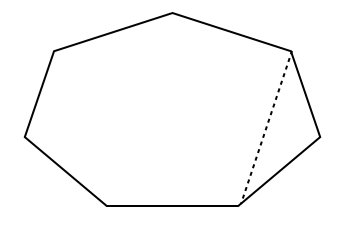
\includegraphics [scale=0.5] {polygon.png} \end{center}

The first part of the answer is to guess. 

\begin{center} 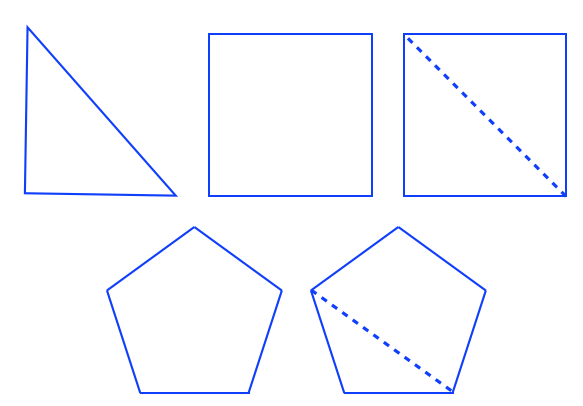
\includegraphics [scale=0.5] {geometrical_induction.png} \end{center}

We know that for a triangle ($n = 3$), the sum of the angles is $180^\circ$, and that the sum does not depend on whether the triangle is acute, right or obtuse.  

Continuing with the square ($n = 4$), we can draw the diagonal and observe that the sum of all the angles is twice  $180^\circ$ or  $360^\circ$.  The partition into two triangles can be carried out with any quadrilateral, it does not require any sides being equal.

From this we guess that the formula may be:
\[ S_n = (n - 2) \cdot 180 \]

And indeed, in going from $n=4$ to $n=5$ sides we can think of the pentagon as being a quadrilateral with an extra triangle.  

And in the first figure, you can see that by adding the extra vertex to go to the $n+1$-gon, we added a triangle, or perhaps you'd rather say than in going from $n+1$ to $n$ we lost a triangle.  

In all cases, the difference between $n$ and $n+1$ is $180^\circ$.  The difference between having $n$ sides and $n+1$ sides is to add $180^\circ$.  The formula seems to work.

We can use induction to \emph{prove} that it is correct.

The proof has two parts.  We must verify the formula for a base case like the triangle, which we've done.  You may wish to check that it works for the square as well, but that's not strictly necessary.

The second part of the proof is to verify that in going from $n$ to $n+1$, we add another $180^\circ$.  \[ (n-2)180^\circ + 180^\circ \stackrel{?}{=} ((n+1)-2)180^\circ \]

On the left-hand side, we have the sum of angles for $n$ sides, which we assume is correct, and then we just add $180^\circ$ to it.  On the right, we have substituted $n+1$ into the formula.

Now we need to show that these are equivalent.  But of course
\[ (n-2)x + x = ((n+1)-2) x \]
\[ n - 2 + 1 = n + 1 - 2 \]
$\square$

\subsection*{Towers of Hanoi}
\begin{center} 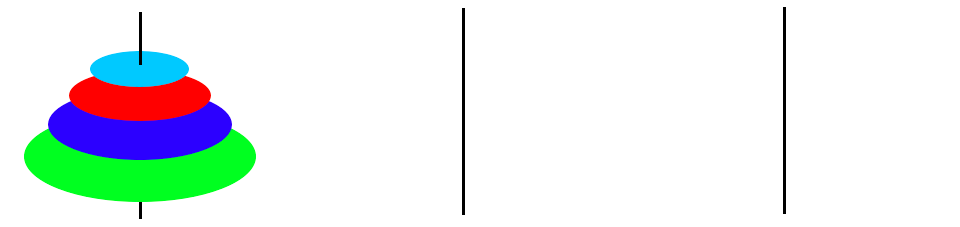
\includegraphics [scale=0.3] {towers.png} \end{center}

In this famous game the goal is to move a set of disks from one peg to another, let us choose the one on the right.  

\url{https://en.wikipedia.org/wiki/Tower_of_Hanoi}

The rules are:

$\circ$ \ Only one disk may be moved at a time.

$\circ$ \ Each move consists of taking the upper disk from one of the pegs and sliding it onto another peg, on top of the other disks that may already be present on that peg.

$\circ$ \ No disk may be placed on top of a smaller disk.

Here is an intermediate stage of the game:
\begin{center} 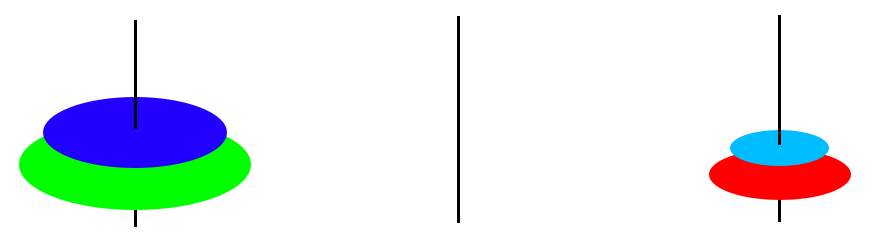
\includegraphics [scale=0.3] {towers2.png} \end{center}

The next move is to place the blue disk on the middle peg.  We can prove that it is possible to move a series of disks of any size from one peg to another.  

We use induction.  

Start from the first position:
\begin{center} 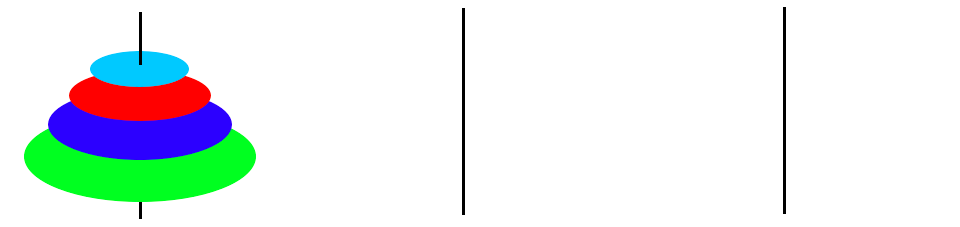
\includegraphics [scale=0.3] {towers.png} \end{center}

Suppose we know how to move $n-1$ disks from one peg to another.  Move them to the middle peg, then move the nth disk to the right peg, then place all the $n-1$ disks on top.  We have moved $n$ disks.

The base case is to move the single light blue disk.  Which peg is to be moved at each stage is shown in this graphic:
\begin{center} 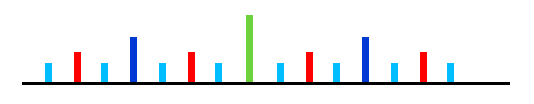
\includegraphics [scale=0.5] {towers3.png} \end{center}

\begin{quote}The puzzle was invented by the French mathematician Édouard Lucas in 1883. There is a legend about a Vietnamese temple which contains a large room with three time-worn posts in it surrounded by 64 golden disks. The monks of Hanoi, acting out the command of an ancient prophecy, have been moving these disks, in accordance with the rules of the puzzle, since that time. The puzzle is therefore also known as the Tower of Brahma puzzle. According to the legend, when the last move of the puzzle is completed, the world will end.\end{quote}

\subsection*{summary}

We can visualize an inductive proof as a kind of chain.  We show that the base case is true, for some value of $n$.  Then we show that if the formula works for $n$ , it must work for $n+1$.

\begin{quote}Mathematical induction proves that we can climb as high as we like on a ladder, by proving that we can climb onto the bottom rung (the basis) and that from each rung we can climb up to the next one (the step).\end{quote}

- Graham, Knuth and Patashnik

[ There is a variant called \emph{strong} induction where we know some statement is true for \emph{all} $0 < k \le n$ and use it to prove something about $n+1$. ]

A few more examples:

\subsection*{sum of digits and divisibility}

It is very easy to check whether any number $n$ is divisible by $9$.  Simply add up all the digits of say, $234783738$:
\[ 2 + 3 + 4 + 7 + 8 + 3 + 7 + 3 + 8 \]
\[ = 5 + 1 + 1 + 1 + 1 + 1 + 0 + 8 \]
\[ = 1 + 8 = 9 \]
Yes, $234783738$ is a multiple of $9$.

We propose that

$9 | (10^n - 1)$ for all integers $n \ge 0$.  

The statement $9|n$ means "9 divides n".

Suppose we know that $9 | 10^k - 1$ for some $n$. We mean that
\[ 10^k - 1 = 9x \]
for some $x$.  Multiply by $10$:
\[ 10 \cdot (10^k - 1) = 10 \cdot 9x \]
\[ 10^{k+1} - 10 = 9 \cdot 10x \]
\[ 10^{k+1} - 1 = 9 \cdot 10x + 9 = 9(10x + 1) \]
The right-hand side is clearly divisible by $9$, and then so is the left-hand side.

The base case is $9|0$ which is true by definition but may be confusing.  Try $n=1$, then $9|(10 -1)$ is certainly correct.

$\square$

Given this, it is easy to show that the sum of digits method always works.

It is worth pointing out that similar reasoning applies to divisibility by $3$.  For any $k$
\[ 10^k - 1 = 3x \]
there exists some $x$ with this property.

So consider the decimal number:
\[ abcd = a \cdot 10^3 + b \cdot 10^2 + c \cdot 10^1 + d \]
\[ = a \cdot (999 + 1) + b \cdot (99+1) + c \cdot (9+1) + d \]
\[ = a \cdot 999 + b \cdot 99 + c \cdot 9 + a + b + c + d \]

Upon division by $9$ or by $3$ the first four terms leave no remainder.  To find the remainder then, we must simply divide $a + b + c + d$ by $9$ or by $3$.  And this is the sum of digits method.

\subsection*{Odd number theorem}

\label{sec:odd_number_theorem}

Here is a simple but very useful inductive proof.

The \emph{odd number theorem} says that the sum of the first $n$ odd numbers is equal to $n^2$.  Here is a "proof without words".

\begin{center} 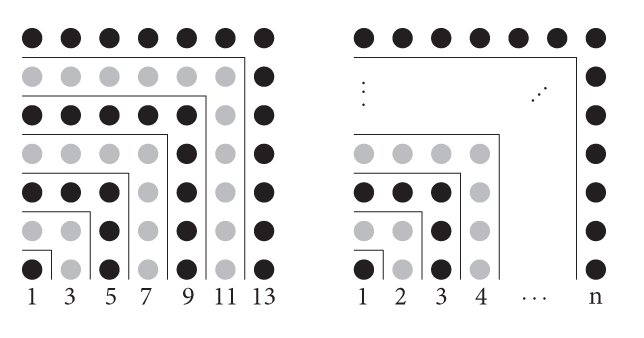
\includegraphics [scale=0.4] {odd_number_theorem.png} \end{center}

We prove this by induction.

\[ \ (0 \times 2 + 1) +  (1 \times 2 + 1) + (2 \times 2 + 1) + (\dots \]
\[ \dots + (n-1) \times 2 + 1) = n^2 \]

Notice that the $n$th odd number is $2 \times (n-1) + 1$.

Our formula says that
\[ 1 + 3 + 5 + \dots + (2n - 1) = n^2 \]
If you like the summation style:
\[ \sum_{k=0}^n 2k - 1 = n^2 \]

As an example, the first five odd numbers are
\[ 1 + 3 + 5 + 7 + 9 = 25 = 5^2 \]

So, if we consider the next odd number, $n$ changes to $n+1$.  The left-hand side gets another term:  we add $2 \times (n+1)-1$ to it.  That is equal to $2n + 1$.

To maintain the equality, add the same quantity to the right-hand side:
\[ n^2 + 2n + 1 = (n+1)^2 \]
Rearrange the result, and that's our formula back again.  We have proved the inductive step.  

To finish, note that the base case is simply
\[ 1 = 1^2 \]
$\square$

The binomial theorem gives the cofactors for a binomial expansion like:
\[ (a + b)^5 = a^5 + 5ab^4 + 10a^2b3 + 10a^3b^2 + 5a^4b + b^5 \]

We will prove this theorem using induction \hyperref[sec:binomial]{\textbf{here}}.

\subsection*{proof of induction}

According to Hamming, if you are not convinced by the ladder analogy, here is another proof that induction works:

\begin{quote}Suppose the statement is not true for every positive (non-negative) integer.  Then there are some false cases.  Consider the set for which the statement is false.  \emph{If} this is a non-empty set, then it would have a least integer, which is $m$.  Now consider the preceeding case, which is $m - 1$.  This $(m-1)$th case must be true by definition, and we know that there is such a case because as a basis for the induction we showed that there was at least one true case.  We now apply the step forward, starting from this true case $m-1$, and conclude that the next case, case $m$, must be true.  But we assumed that it was \emph{false}!  A contradiction. \end{quote}

Therefore, there are no false cases.

$\square$

\end{document}  